\documentclass{article}
\usepackage{listings}
\usepackage{xcolor}
\usepackage{amsmath}
\usepackage{hyperref}
\usepackage{enumitem}
\usepackage{geometry}
\usepackage{graphicx}
\usepackage[table]{xcolor}
\usepackage{tikz}
\usetikzlibrary{positioning}
\geometry{margin=1in}

\title{Functions}
\author{}
\date{}

\definecolor{codegray}{rgb}{0.5,0.5,0.5}
\definecolor{backcolour}{rgb}{0.95,0.95,0.92}

\lstdefinestyle{cppstyle}{
  backgroundcolor=\color{backcolour},
  commentstyle=\color{codegray},
  keywordstyle=\color{blue},
  numberstyle=\tiny\color{codegray},
  stringstyle=\color{red},
  basicstyle=\ttfamily\footnotesize,
  breakatwhitespace=false,
  breaklines=true,
  captionpos=b,
  keepspaces=true,
  numbers=none,
  numbersep=5pt,
  showspaces=false,
  showstringspaces=false,
  showtabs=false,
  tabsize=2,
  language=C++
}

\begin{document}

\maketitle


Functions allow you to group reusable blocks of code and break programs into logical parts.

\section{What is a Function?}

A function is a named block of code that performs a specific task. Functions help with code reuse, readability, and modularity.

\section{Defining and Calling a Function}

\begin{lstlisting}[style=cppstyle]
void greet() {
    cout << "Hello!\n";
}

int main() {
    greet();  // function call
    return 0;
}
\end{lstlisting}

\subsection{Functions with Parameters}

\textbf{Pass-by-Value:} A copy of the variable is passed. Changes inside the function do \textbf{not} affect the original.

\begin{lstlisting}[style=cppstyle]
void square(int x) {
    x = x * x;
    cout << "Inside function: " << x << endl;
}

int main() {
    int num = 5;
    square(num);
    cout << "After function: " << num << endl;  // still 5
}
\end{lstlisting}

\textbf{Pass-by-Reference:} The actual variable is passed using \texttt{\&}. Changes inside the function \textbf{do} affect the original.

\begin{lstlisting}[style=cppstyle]
void doubleValue(int &n) {
    n = n * 2;
    cout << "Inside function: " << n << endl;
}

int main() {
    int num = 5;
    doubleValue(num);
    cout << "After function: " << num << endl;  // now 10
}
\end{lstlisting}

\textbf{Summary:}
\begin{itemize}
    \item Use \textbf{pass-by-value} when you don't want the function to change the original variable.
    \item Use \textbf{pass-by-reference} when the function should modify the original variable.
\end{itemize}

\section{Function Prototypes}

Prototypes tell the compiler about a function before its actual definition.

\begin{lstlisting}[style=cppstyle]
int add(int, int);  // prototype

int main() {
    cout << add(2, 3);
}

int add(int a, int b) {
    return a + b;
}
\end{lstlisting}

\section{Scope of Variables}

Variables can be declared globally (outside any function) or locally (inside a function). Local variables exist only within their function.

\textbf{Scope Diagram:}
\begin{center}
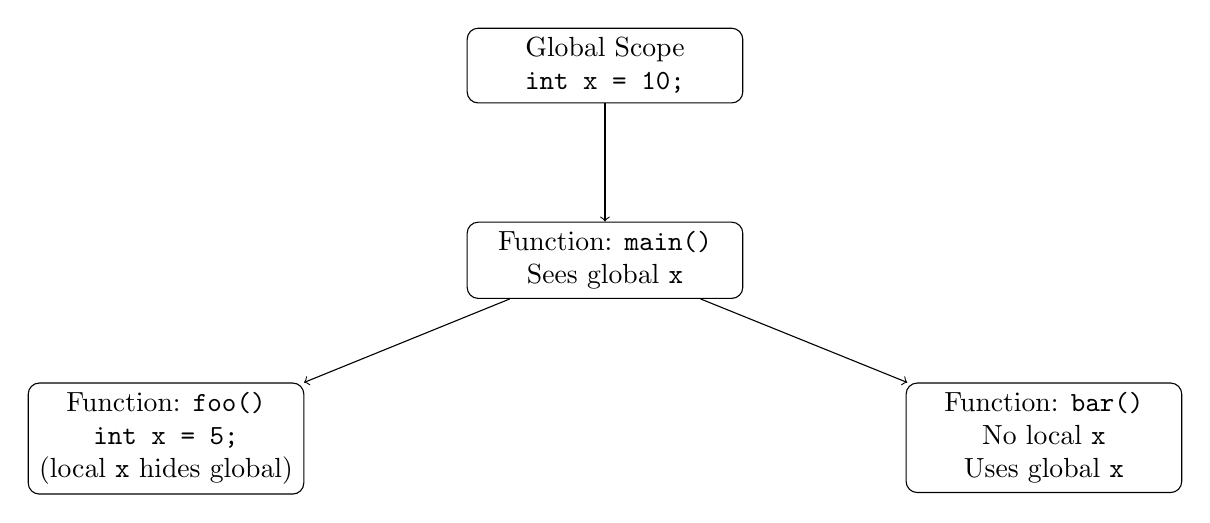
\begin{tikzpicture}[node distance=1.5cm, every node/.style={draw, rectangle, rounded corners, align=center, minimum width=3.5cm}]
    \node (global) {Global Scope\\ \texttt{int x = 10;}};
    \node (main) [below=of global] {Function: \texttt{main()}\\ Sees global \texttt{x}};
    \node (foo) [below left=of main, xshift=-1cm] {Function: \texttt{foo()}\\ \texttt{int x = 5;}\\ (local \texttt{x} hides global)};
    \node (bar) [below right=of main, xshift=1cm] {Function: \texttt{bar()}\\ No local \texttt{x} \\ Uses global \texttt{x}};

    \draw[->] (global) -- (main);
    \draw[->] (main) -- (foo);
    \draw[->] (main) -- (bar);
\end{tikzpicture}
\end{center}

\section{Void vs Non-Void Functions}

- \texttt{void} functions do not return a value.
- Non-void functions specify a return type like \texttt{int} or \texttt{double}.

\begin{lstlisting}[style=cppstyle]
void sayHi() {
    cout << "Hi!\n";
}

int getFive() {
    return 5;
}
\end{lstlisting}

\end{document}